\chapter{Technical system overview}
\section{System}
The following section describes the phantom following \cite{van2011modeling}'s methodology.
\subsection{Organ}
The organ to be simulated is the myocardium of the left ventricle, more specifically the blood flow in the myocardium. The left ventricle has a \ac{HLA} and \ac{VLA} cross-sectional shape of a horseshoe and a \ac{SA} cross-sectional shape of a circle, see figure \ref{fig:ventricle_shapes}. Quantitative data on blood flow is available in previous research by \cite{uren1994relation, chiribiri2013normal, ho2014dynamic, slart2015Pres}. Heart size indications are available in previous research by \cite{lin2008cardiac, maceira2006normalizedleft, maceira2006normalizedright}.

\begin{figure}[H]
	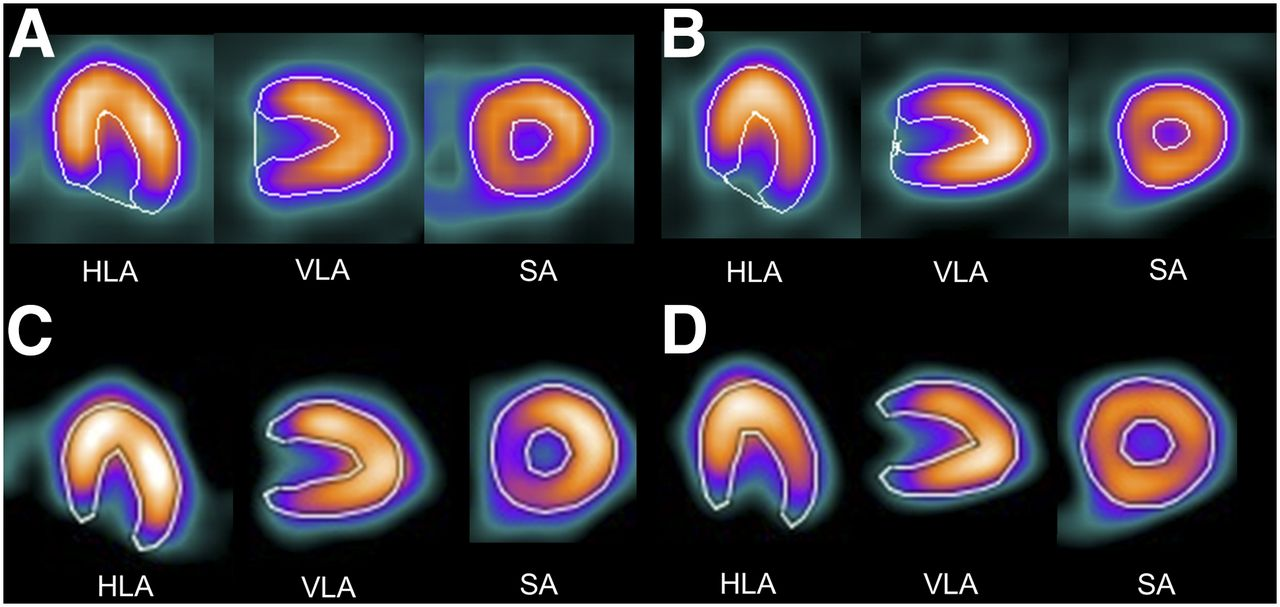
\includegraphics[scale=1]{./images/ventricle_shapes.jpg}
	\caption{Ventricle shapes in different planes\citep{yoneyama2017validation}}
	\label{fig:ventricle_shapes}
\end{figure}

\subsection{Population}
The heart phantom will be designed for average adults of both genders with ages between 18 and 79. The population consisted of patients with and without \ac{CAD}.
\subsection{Physiological states}
The heart will be simulated in both a resting state and in a stress state while the "patient" is in a supine position. The D-SPECT captures intensity images based on gamma rays caused by the radioactive decay of a tracer which is injected intravenously. The D-SPECT does not capture any information other than intensity information from gamma rays. Therefore the composition of the fluid is of less importance making water most practical.
\subsection{Pathologies}
The phantom aims to simulate the perfusion in the myocardium of healthy patients and of patients with \ac{CAD}, more specifically stenosis of the coronary arteries or its subsequent branches. Stenosis in one of the arteries will have an impact on the overall flow behaviour (higher pressure, less overall flow, more flow to non-stenotic arteries) and thus requires the phantom to mimic the same behaviour.
\subsection{Clinical signs and monitored variables}
Blood flow is the most important variable to be monitored as these will be compared to the quantitative results produces by the processing software of the D-SPECT's images. Blood pressure must be monitored for indicative purposes. Depending on the phantom's final design, blood pressure can be critical for the simulation of the myocardial perfusion.
\subsection{Critical incidents}
No critical incidents will be simulated.
\subsection{Interventions}
No interventions will be simulated.
\subsection{Overall block diagram}
Figure \ref{fig:overall_block} shows an overview of all systems, how they are separated, and their interrelations. A distinction is made between four key elements; the flow set-up, the phantom, the imaging system, and external systems. The generation of an artificial heartbeat and the injection of the tracer are carried out externally and do not require development. Additionally, the imaging system (D-SPECT) with analysis software (4DM) do not require development since it concerns off-the-shelf hard-/software. The flow set-up and the phantom do require development. 

The flow is generated for different physiological states for high and low flows, i.e. for stress and rest. A closed-loop circuit monitors and controls the flow for optimal accuracy. The tracer is injected and flows to the phantom where the myocardial perfusion is mimicked. The contaminated water flows out of the phantom such that it can de disposed. Optionally, if the tracer can be filtered from the contaminated water, a closed, recirculating system can be fabricated; greatly reducing water waste. The tracer undergoes radioactive decay that results in the emission of gamma rays, which are picked up by the D-SPECT's detectors. The resulting intensity images can be reconstructed to form cross-sectional images which in turn are used to quantify the blood flow.

\begin{figure}[H]
	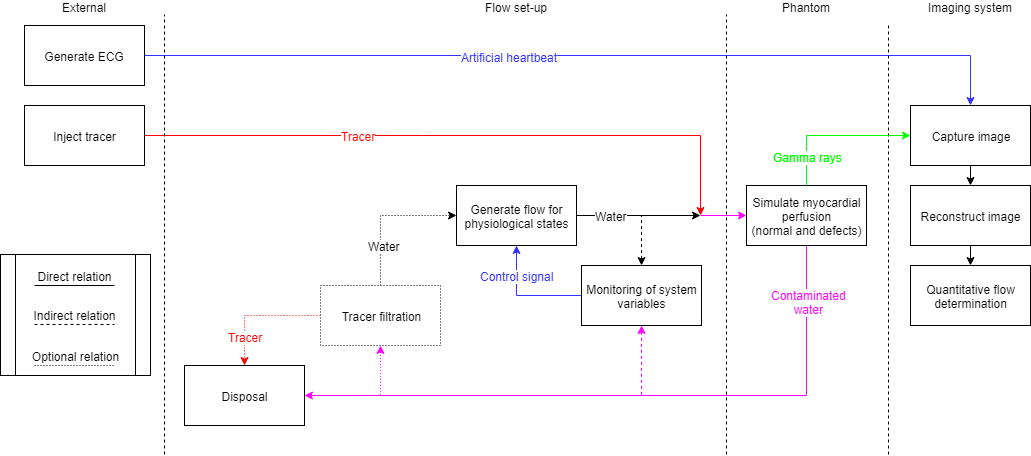
\includegraphics[width=\linewidth]{./images/technical_blockdiagram.png}
	\caption{Overall block diagram}
	\label{fig:overall_block}
\end{figure}

\section{Function requirements}
This section specifies the requirements set for the functions mentioned in figure \ref{fig:funcarch}.
\subsection{Generate flow}
In the project plan, a literature overview is given on perfusion phantoms, for a variety of organs, but also on physiological factors: perfusion rates, blood pressures, rates of stenosis et cetera. The TFR-GF requirements are based on the estimates by \cite{uren1994relation}, summarised in appendix \ref{app:physoverview}, \cite{chiribiri2013normal}, \cite{ho2014dynamic}, summarised in appendix \ref{app:physoverview_ho}, and \cite{slart2015Pres}.

Decisions and design choices are given in table \ref{tab:genflow_text}, quantitative requirements are given in table \ref{tab:genflow_quan}.

\begin{table}[H]
\caption{Textual requirements for function: Generate flow}
\label{tab:genflow_text}
\begin{tabular}{p{25mm}|p{115mm}|}
	\textbf{Requirement number} & \multicolumn{1}{c}{\textbf{Description}} \\
	\hline
	TFR-GFT01 & A variable, but constant, flow is to be generated, i.e. non-pulsatile. \\
	TFR-GFT02 & Flow generators need to be interchangeable. \\
	TFR-GFT03 & Flow feedback control for flow generators. \\
	\cline{2-2}
\end{tabular}
\end{table}

\textbf{TFR-GFT01} is based on reducing the complexity of the set-up. The ROI based AIF averages the intensity over time, which removes the pulsatile nature. Furthermore, the heart rate cannot be determine in the measurements results. Therefore, pulsatile flow is not a priority.
\textbf{TFR-GFT02} is based on maintaining flexibility such that the most optimal flow generator can be chosen based on the requirements for a specific experiment.

\textbf{TFR-GFT03} is based on ensuring reliability; no validation can be performed when the flow is not controlled.

\begin{table}[H]
\caption{Quantitative requirements for function: Generate flow}
\label{tab:genflow_quan}
\begin{tabular}{p{24mm}|p{65mm}ccp{21mm}|}
	\textbf{Requirement number} & \multicolumn{1}{c}{\textbf{Description}} & \multicolumn{1}{c}{ } & \multicolumn{1}{c}{\textbf{Value}} & \multicolumn{1}{c}{\textbf{Unit}} \\
	\hline
	TFR-GFQ01*	& Upper limit myocardial perfusion. 		 		& = 				& 300 				&  mL/min/100g \\
	TFR-GFQ02* 	& Lower limit myocardial perfusion. 				& = 				& 60 				& mL/min/100g \\
	TFR-GFQ03* 	& Typical perfusion rate during stress. 	 		& > \spacing < 		& 190 \spacing 300 	& mL/min/100g \\
	TFR-GFQ04*  	& Typical perfusion rate during rest. 			& > \spacing < 		& 60 \spacing 95 	& mL/min/100g \\
	TFR-GFQ05**	& Upper limit cardiac output.				 		& =					& 5 				& L/min \\
	\sout{TFR-GFQ06+}		& \sout{Lower limit arterial pressure.}			& \sout{=}					& \sout{56}			& \sout{mmHg} \\
	\sout{TFR-GFQ07+}		& \sout{Upper limit arterial pressure.}				& \sout{=} 				& \sout{155}				&\sout{mmHg} \\
	\sout{TFR-GFQ08}		& \sout{Mean Arterial Pressure (MAP)}\footnotemark. 	& \sout{=} 				& \sout{89}				&\sout{mmHg} \\
	\sout{TFR-GFQ09}		& \sout{Typical MAP.}								 	& \sout{> \spacing <}		& \sout{\invchar 70 \spacing 110}	& \sout{mmHg} \\
	TFR-GFQ10 	& Feedback control accuracy 						& =					& 5					& \% \\
	\cline{2-5}
\end{tabular} \\
\raggedright
\textit{* combined flow to myocardium, indicated by blue arrows in figure \ref{fig:sim_heart}.} \\
\textit{** flow \textbf{not} entering the myocardium, indicated by red arrow in figure \ref{fig:sim_heart}.} \\
\sout{\textit{+ based on diastolic and systolic blood pressures, respectively. Measured at dashed line P in figure \ref{fig:sim_heart}.}}
\end{table}

\footnotetext{Calculated as: $MAP \simeq DP + \sfrac{1}{3} (SP-DP)$}

\begin{figure}
\centering
\begin{minipage}{.5\textwidth}
  \centering
  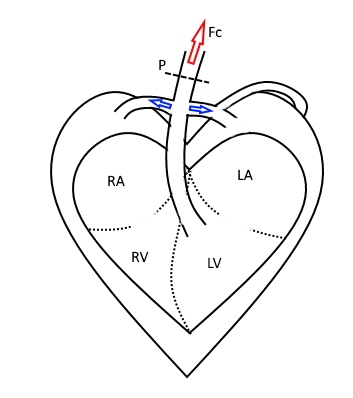
\includegraphics[width=0.7\linewidth]{./images/simplified_heart.png}
  \captionof{figure}{Simplified, schematic overview of the heart.}
  \label{fig:sim_heart}
\end{minipage}%
\begin{minipage}{.5\textwidth}
  \centering
  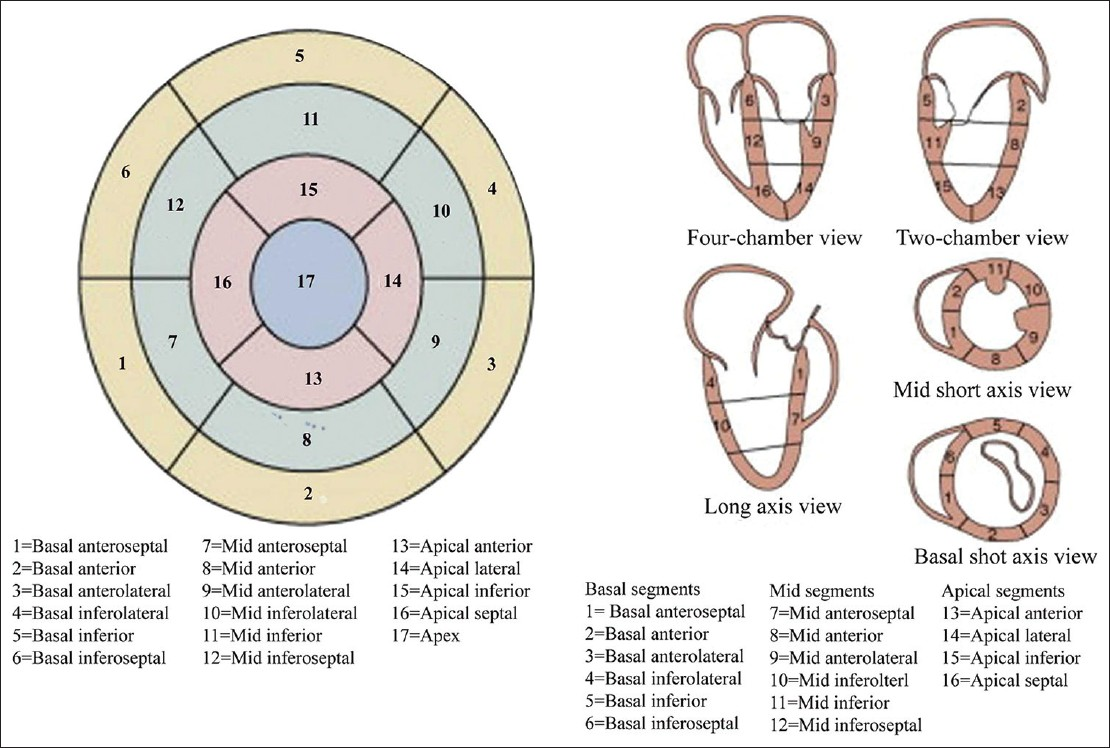
\includegraphics[width=0.95\linewidth]{./images/17_segment.jpg}
  \captionof{figure}{17-segment heart model (\citep{muralidhar2013practice} based on \citep{american2002standardized}}
  \label{fig:segment_heart}
\end{minipage}
\end{figure}

\subsection{Measuring flow and pressure}
This section focusses on the requirements for the measuring of the system variables; flow and pressure.
\begin{table}[H]
\caption{Quantitative requirements for function: Measure flow and pressure}
\label{tab:measflow_quan}
\begin{tabular}{p{25mm}|p{65mm}ccp{20mm}|}
	\textbf{Requirement number} & \multicolumn{1}{c}{\textbf{Description}} & \multicolumn{1}{c}{ } & \multicolumn{1}{c}{\textbf{Value}} & \multicolumn{1}{c}{\textbf{Unit}} \\
	\hline
	TFR-MFPQ01	& Flow measuring accuracy. 		 			 & <= 		& 5 		& \% \\
	TFR-MFPQ02 	& Pressure measuring accuracy.		 		 & <= 		& 5 		& \% \\
	TFR-MFPQ03 	& Absolute flow resolution.				 	 & >=	 	& 1 		& mL/min \\
	TFR-MFPQ04  & Sampling rate.					 		 & >= 		& 10 		& Hz \\
	\cline{2-5}
\end{tabular} \\
\raggedright
\end{table}

\begin{figure}[H]
	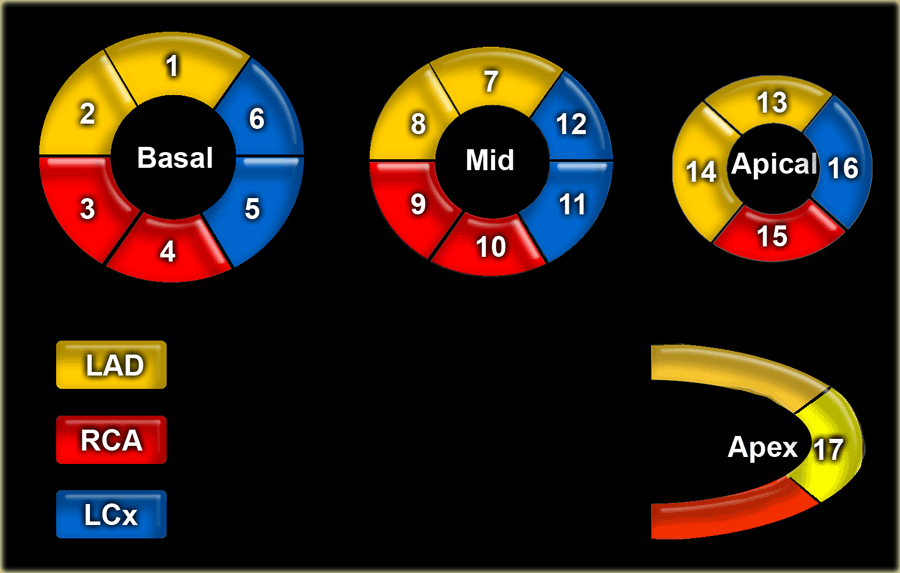
\includegraphics[width=0.5\linewidth]{./images/17_supply.png}
	\caption{Schematic representation of the supply to each segment (simplified)\citep{es2009simple}.}
	\label{fig:segment_supply}
\end{figure}

\begin{figure}[H]
	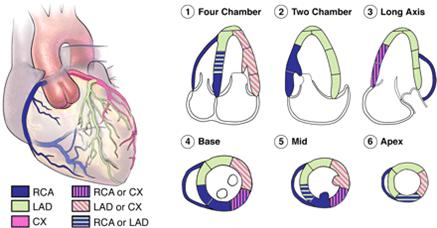
\includegraphics[width=0.5\linewidth]{./images/17_segment_2.jpg}
	\caption{Schematic representation of the supply to each segment\citep{american2002standardized}.}
	\label{fig:segment_supply2}
\end{figure}

\subsection{Simulate myocardial perfusion}
This section specifies the requirements for the simulation of the myocardial perfusion.
\begin{table} [H]
\caption{Function requirements for function: Simulate myocardial perfusion}
\label{tab:funcsim}
\begin{tabular}{l|p{120mm}|}
	\makecell[l]{\textbf{Requirement} \\  \textbf{number}} & \multicolumn{1}{c}{\textbf{Description}}\\
	\hline
	\sout{TFR-SIMT01} & \sout{An \ac{AIF} must be extractable from the left ventricle, as per software requirement.}\\
	TFR-SIM02 & Stenotic arteries are mimicked in a physiological way by physically narrowing (or increasing flow resistance) of certain arteries. \\
	TFR-SIMT03 & Different stenotic severity, should be possible by, for example, variable flow resistors or interchanging components. \\
	TFR-SIMT04 & The phantom must be compatible with D-SPECT protocol. \\
	\hspace{1.5cm} A) & Flow to the myocardium is supplied by the RCA, LAD, and LCx. \\
	\hspace{1.5cm} B) & Flow for each segment is supplied individually by branches of the RCA, LAD, and LCx, see figure \ref{fig:segment_supply}. \\
	\hspace{1.5cm} C) & Flow from each segment is measured separately such that they can be compared to the 17-segment model. \\
	\hspace{1.5cm} D) & An ROI for the AIF can be taken in the left atrium. Alternatively, the ROI for the AIF can be taken in the left ventricle. \\
	\hspace{1.5cm} \sout{E)} & \sout{An AIF can be taken from the left atrium.} \\
	\hspace{1.5cm} \sout{F)} & \sout{The left ventricle's myocardium has a Vertical and Horizontal Longitudinal Axial (VLA/HLA) cross-sectional shape of a horseshoe.} \\
	\hspace{1.5cm} \sout{G)} & \sout{The left ventricle's myocardium has a Short Axial (SA) cross-sectional shape of a circle.} \\
	\hspace{1.5cm} H) & The phantom is oriented such that it mimics a patient in supine position. \\
	TFR-SIMT05* & Phantom's compartment model should match the currently practised protocol.\\
	\hspace{1.5cm} A) & The tracer specified in section \ref{sec:inj_tracer}.\\
	\hspace{1.5cm} B) & The contrast agent is absorbed by the myocardium to approximately 1.2\% of administered activity in 5 minutes. \\
	\hspace{1.5cm} C) & Contrast accumulates in skeletal muscles, spleen, liver, and kidneys (potential interference). \\
	\cline{2-2}
\end{tabular}
\raggedright
\textit{* \url{https://pubchem.ncbi.nlm.nih.gov/compound/131704316\#section=Absorption-Distribution-and-Excretion}}
\end{table}

\textbf{TFR-SIMT02} is based on the assumption that the relation between arteries, especially when some are narrowed, is too complex to be modelled independently. Simply reducing the overall flow in the myocardium will not capture that relation. Each segment of the left ventricle is supplied by a different branch of the three coronary arteries. One narrowed branch will have an impact on \textit{all} other branches, which leads to \textbf{TFR-SIMT03}. The severity of the stenosis will impact the other branches differently.

\textbf{TFR-SIMT04} is based on the goal of the project; to validate the D-SPECT. As mentioned in section \ref{sec:concept_oper}, the relatively less expensive, less invasive (patient friendliness and dose reduction), faster and more accurate system makes it suitable for myocardial perfusion imaging. However, the quantitative nature of the dynamic scanning protocol requires validation since it has not been carried out. Furthermore, the learning, educational, and training purposes of the phantom study is desired by researchers, manufacturers, and medical personnel. This is somewhat extended by \textbf{TFR-SIMT05}. Protocols already exist within clinics and is therefore the best starting point for research and phantom development.

\subsection{Inject tracer}
\label{sec:inj_tracer}
The injection of tracer into the flow set-up, is carried out by an external infusion pump. 

\begin{table}[H]
\caption{Textual requirements for function: Inject tracer}
\label{tab:injtrac_text}
\begin{tabular}{l|p{115mm}|}
	\makecell[l]{\textbf{Requirement} \\  \textbf{number}} & \multicolumn{1}{c}{\textbf{Description}} \\
	\hline
	TFR-ICT01 			& Tracer volume is variable. \\
	TFR-ICT02			& Tracer activity is variable, also see TFR-ICQ03. \\
	\sout{TFR-ICT03}			& \sout{Tracer agent is variable.} \\
	TFR-ICT04 			& Tracer injection is reproducible, also see TFR-ICT05.\\
	TFR-ICT05 			& Tracer protocol should match the currently practised protocol. \\
	\hspace{1.5cm} A) 	& See TFR-ICQ01. \\
	\hspace{1.5cm} \sout{B)} 	& \sout{Tracer is injected, as bolus, via infusion pump.} \\
	\hspace{1.5cm} \sout{C)} 	& \sout{A pre-bolus is to precede the main bolus.} \\
	\cline{2-2}
\end{tabular}
\end{table}

\textbf{TFR-ICT01} through \textbf{TFR-ICT03} are defined such that the tracer protocol can be optimised by performing experiments with different volumes, activity, or tracers. However, the first experiments will focus on the currently practised protocol, as is stated in \textbf{TFR-ICT05}. \textbf{TFR-ICT04} is based on the first experiments performed at the ZGT, Hengelo, where it is concluded that manual injection is not reproducible and results in unreliable results. These effect are directly visible in the dynamic scans. Therefore, an infusion pump is to be used.

\begin{table}[H]
\caption{Quantitative requirements for function: Inject tracer}
\label{tab:injtrac_quan}
\begin{tabular}{l|p{65mm}ccp{20mm}|}
	\makecell[l]{\textbf{Requirement} \\  \textbf{number}} & \multicolumn{1}{c}{\textbf{Description}} & \multicolumn{1}{c}{ } & \multicolumn{1}{c}{\textbf{Value}} & \multicolumn{1}{c}{\textbf{Unit}} \\
	\hline
	TFR-ICQ01 	& Tracer to be used. 					& = 			& \multicolumn{2}{p{35mm}|}{Technetium (\textsuperscript{99m}Tc) Tetrofosmin} \\
	\sout{TFR-ICQ02} 	& \sout{Pre-bolus activity.}					& \sout{=} 			& \sout{37}				& \sout{Mega Becquerel} \\
	TFR-ICQ03*	& Typical main bolus activity.		 	& > \spacing < 	& 500 \spacing 700 	& Mega Becquerel \\
	TFR-ICQ04+	& Typical main bolus volume. 			& > \spacing <	& 1 \spacing 2 		& Millilitre \\
	TFR-ICQ05+	& Typical main bolus injection speed.	& > \spacing < 	& 1 \spacing 2		& Millilitre per second \\
	TFR-ICQ06+	& Saline flush after tracer injection.	& =				& 30				& Millilitre \\
	\cline{2-5}
\end{tabular} \\
\raggedright
\textit{* hefty patient tend to get higher activity injected, i.e. 700 MBq.} \\
\textit{+ based on D-SPECT manufacturer's specification and current clinical protocol.}
\end{table}

\section{Physical requirements}
\label{sec:phys_req}
\rrow{Determine size of seating of D-SPECT}
\rrod{Determine weight limit of seating of D-SPECT}
\rrod{Must it be completely anatomical? Discuss with Kees}
\rrow{Adjust requirements if the phantom does not have to be anatomical. Kees does not feel that it is necessary to have four chambers. However, the myocardial shape is still debateable.}
This sections specifies the requirements on the physical aspects of the phantom and flow set-up, a.o. sizes, dimensions.

\begin{table}[H]
\caption{Physical requirements (textual)}
\label{tab:physrec_text}
\begin{tabular}{l|p{115mm}|}
	\makecell[l]{\textbf{Requirement} \\  \textbf{number}} & \multicolumn{1}{c}{\textbf{Description}} \\
	\hline
	TR-PRT01 			& The phantom's left ventricle is to be placed inside the QRM TRX-116, see TR-PRQ01. \\
	TR-PRT02 			& The phantom's left ventricle must fit in the D-SPECT's imaging area. \\
	TR-PRT03 			& The phantom must be anatomically shaped. \\
	\hspace{1.5cm} \sout{A)} 	& \sout{In correspondence with requirements TFR-SIMT04.} \\
	\hspace{1.5cm} \sout{B)} 	& \sout{Four chambered phantom that correspond to left/right ventricle and left/right atrium.} \\
	\hspace{1.5cm} C) 	& Segmented myocardium surrounds heart chambers. \\
	\hspace{1.5cm}\sout{D)}	& \sout{Three coronary arteries, RCA, LAD and LCx, supply the myocardium.} \\
	\hspace{1.5cm} E) 	& The coronary arteries run outside of the myocardium. \\
	\hspace{1.5cm} F) 	& The coronary veins run outside of the myocardium. \\
	\hspace{1.5cm} G) 	& The left ventricle's myocardium has a Vertical and Horizontal Longitudinal Axial (VLA/HLA) cross-sectional shape of a horseshoe. \\
	\hspace{1.5cm} H) 	& The left ventricle's myocardium has a Short Axial (SA) cross-sectional shape of a circle. \\
	TR-PRT04 			& The flow set-up is to remain horizontal (preventing additional flow resistance). \\
	TR-PRT05 			& The phantom must be easily be cleared of air bubbles. \\
	\cline{2-2}
\end{tabular}
\end{table}

\textbf{TR-PRT01} is based on creating realistic simulation of myocardial perfusion, thereby requiring a thorax phantom (with possible extension rings to simulate more hefty patients). The QRM TRX-116 has been successfully used for CT experiments. The 4DM software looks at the left ventricle thereby requiring the left ventricle to be in the phantom and in the imaging area, as stated in \textbf{TR-PRT02}.

\rrod{Must it be anatomically shaped?}
\rrow{Verify shape of ventricle at webinar}
\textbf{TR-PRT03} is based on the requirements by the 4DM software. It does not require a four chambered heart and as such is no longer a requirement. However, the software must recognise the ventricle and thus imposes physical requirements on the left ventricle of the phantom.

\textbf{TR-PRT04} is based on the choice to prevent unnecessary complexity. Remaining horizontal will negate gravity.

\textbf{TR-PRT05} is based on the attenuation of air, which compromises the TAC determination. The phantom should be easily cleared of air bubbles.

\begin{table}[H]
\caption{Physical requirements (Quantitative)}
\label{tab:physrec_quan}
\begin{tabular}{l|p{65mm}ccp{20mm}|}
	\makecell[l]{\textbf{Requirement} \\  \textbf{number}} & \multicolumn{1}{c}{\textbf{Description}} & \multicolumn{1}{c}{ } & \multicolumn{1}{c}{\textbf{Value}} & \multicolumn{1}{c}{\textbf{Unit}} \\
	\hline	
	TR-PRQ01 & Short Axial diameter.		 						& < 			& 100 							& Millimetre \\
	TR-PRQ02 & Weight on patient chair. 							& < 			& 171 							& Kilogram   \\
	\sout{TR-PRQ03+} & \sout{Phantom's outer dimensions.} 							& 				& 								& 			 \\
	\hspace{1.5cm} \sout{A)} & \sout{Basal-Apical distance.} 						& \sout{$\approx$} 	& \sout{120} 							& \sout{Millimetre} \\
	\hspace{1.5cm} \sout{B)} & \sout{Left-Right Lateral distance.}				& \sout{$\approx$} 	& \sout{80}							& \sout{Millimetre} \\
	\hspace{1.5cm} \sout{C)} & \sout{Anterior-Posterior distance}. 				& \sout{$\approx$} 	& \sout{60}							& \sout{Millimetre} \\
	TR-PRQ04++ & Left ventricle dimensions.							& 				& 								& 			 \\
	\hspace{1.5cm} A)* & Internal Apical-Annular distance.			& > \spacing < 	& \invchar 69.4 \spacing 105.8	& Millimetre \\
	\hspace{1.5cm} B) & Internal Septal-Lateral distance. 			& > \spacing <	& 38.2 \spacing 55.6			& Millimetre \\
	\hspace{1.5cm} C) & Internal Anterior-Inferior.					& > \spacing < 	& 46.9 \spacing 68.5 			& Millimetre \\
	\hspace{1.5cm} D) & Myocardial wall thickness.					& > \spacing < 	& 4.8 \spacing 9.8				& Millimetre \\
	\hspace{1.5cm} E)= & Internal volume.							& > \spacing < 	& \invchar 47 \spacing 156 	& Millilitre \\
	\sout{TR-PRQ05++} & \sout{Right ventricle dimensions.}							& 				&								&			 \\
	\hspace{1.5cm} \sout{A)} & \sout{Internal Apical-Annular distance.}			& \sout{> \spacing <}	& \sout{44.8 \spacing 79.2} 			& \sout{Millimetre} \\
	\hspace{1.5cm} \sout{B)} & \sout{Internal Septal-Medial	distance.}			& \sout{> \spacing <} 	& \sout{19.2 \spacing 40.0} 			& \sout{Millimetre} \\
	\hspace{1.5cm} \sout{C)} & \sout{Internal Anterior-Inferior distance.}		& \sout{> \spacing <} 	& \sout{42.2 \spacing 73.6} 			& \sout{Millimetre} \\
	\hspace{1.5cm} \sout{D)} & \sout{Myocardial wall thickness.}					& \sout{> \spacing <}	& \sout{1.0 \spacing 3.8}				& \sout{Millimetre} \\
	\hspace{1.5cm} \sout{E)=} & \sout{Internal volume.} 							& \sout{> \spacing <}	&  \sout{\invchar 24.9 \spacing 163.0} & \sout{Millilitre} \\
	\sout{TR-PRQ06+} 	& \sout{Phantom resembles weight of average human heart.} 	& \sout{> \spacing <}	& \sout{250 \spacing 350} 				& \sout{Gram}\\
	TR-PRQ07	& Flow path height relative to platform (see figure \ref{fig:QRM_thorax} and \ref{fig:QRM_extension}).			& 				&								& \\
	\hspace{1.5cm} A)	& Without extension rings.					& $\approx$ 	& 120 $\pm$ 10					& Millimetre \\
	\hspace{1.5cm} B)	& With extension ring M.					& $\approx$ 	& 145 $\pm$ 10					& Millimetre \\
	\hspace{1.5cm} C) 	& With extension ring L.					& $\approx$		& 170 $\pm$ 10					& Millimetre \\
	\hspace{1.5cm} D)	& With extension ring XL.					& $\approx$		& 245 $\pm$ 10					& Millimetre \\
	\cline{2-5}
\end{tabular} \\
\raggedright
\textit{* Annular $\rightarrow$ Annulus $\rightarrow$ assuming mitral valve level.} \\
\sout{\textit{+ based on OpenStax College (2013).}} \\
\textit{++ based on \cite{lin2008cardiac}.} \\
\textit{= based on \cite{maceira2006normalizedleft} and \cite{maceira2006normalizedright}}
\end{table}

\begin{figure}[H]
\centering
\begin{minipage}{.5\textwidth}
  \centering
  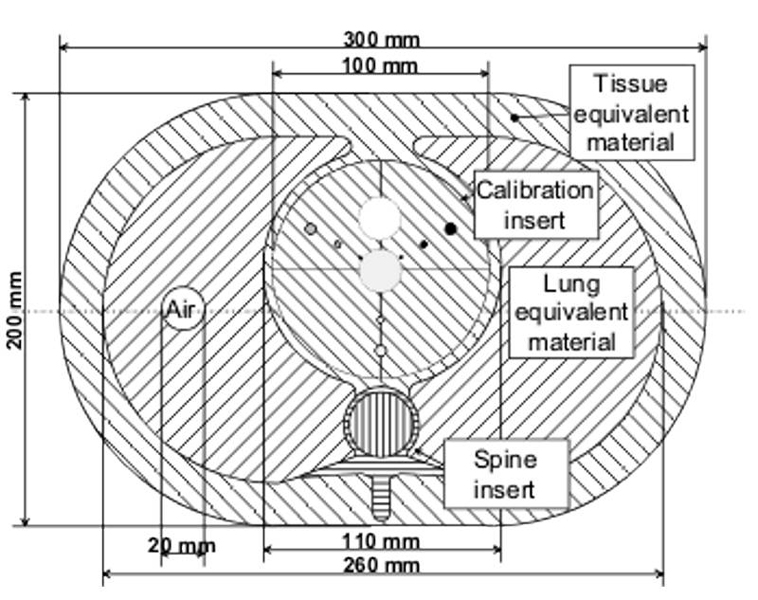
\includegraphics[width=0.95\linewidth]{./images/cardio_2.jpg}
  \captionof{figure}{QRM thorax phantom \citep{QRMthorax}.}
  \label{fig:QRM_thorax}
\end{minipage}%
\begin{minipage}{.5\textwidth}
  \centering
  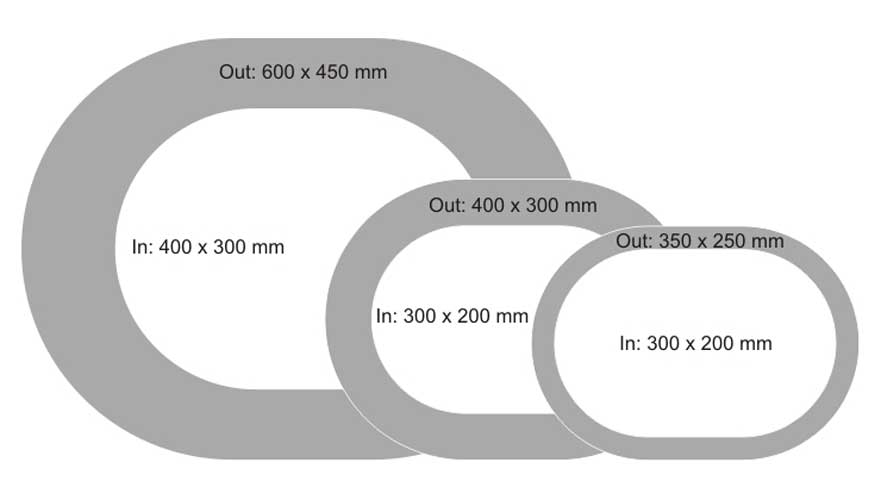
\includegraphics[width=0.95\linewidth]{./images/extension_2.jpg}
  \captionof{figure}{QRM thorax phantom extension rings\citep{QRMextension}.}
  \label{fig:QRM_extension}
\end{minipage}
\end{figure}

\section{External requirements}
\rrot{Determine how much noise output it may have.}
\rrod{Determine the height of the chair of the D-SPECT}
This section specifies the requirements that result from external influences.
\begin{table} [H]
\caption{External requirements (Textual)}
\label{tab:extreq_text}
\begin{tabular}{l|p{120mm}|}
	\makecell[l]{\textbf{Requirement} \\ \textbf{number}} & \multicolumn{1}{c}{\textbf{Description}}\\
	\hline
	TR-ERT01 & No high-density or "High-Z" material is to be used.\\ 
	TR-ERT02 & The phantom's left and front side must remain free, see figure \ref{fig:spect_surround}. \\ 
	\sout{TR-ERT03**} & \sout{Any part of the flow set-up and/or phantom, that does not fit directly on the patient chair, must remain horizontal with the remaining parts between 63 and 93cm.} \\
	\cline{2-2}
\end{tabular}
\raggedright

\end{table}

\begin{figure} [H]
  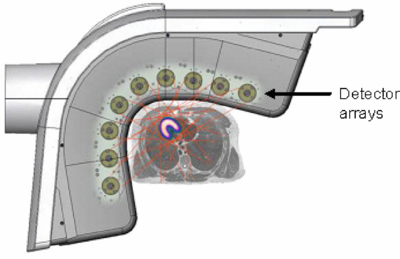
\includegraphics[width=0.5\linewidth]{./images/surrounding_spect.jpg}
  \caption{figure}{Schematic drawing of D-SPECT head\citep{erlandsson2009performance}.}
  \label{fig:spect_surround}
\end{figure}

\textbf{TR-ERT01} is based on material properties; "High-Z", or High-Density, material tend to block gamma radiation emitted by \ac{SPECT} tracers. Some examples of High-Z materials are Titanium (Ti), Chromium (Cr), Vanadium (V), Iron (Fe), or Lead (Pb).

\textbf{TR-ERT02} is based on the D-SPECTS design. The curved design allows for better patient comfort and proper imaging, but will require the phantom for being accessible, i.e. not blocked by High-Z materials, from the patient's left and front side.

\begin{table}[H]
\caption{External requirements (Quantitative)}
\label{tab:extreq_quan}
\begin{tabular}{l|p{65mm}ccp{20mm}|}
	\makecell[l]{\textbf{Requirement} \\  \textbf{number}} & \multicolumn{1}{c}{\textbf{Description}} & \multicolumn{1}{c}{ } & \multicolumn{1}{c}{\textbf{Value}} & \multicolumn{1}{c}{\textbf{Unit}} \\
	\hline	
	TR-ERQ01* &  Electric power. &  &  &  \\
	\hspace{1.5cm} A) & Supply voltage. 	& = 	& 230 	& Volt \\
	\hspace{1.5cm} B) & Supply current at TR-ERQ01 A). 	& < < 	& 6		& Ampere \\
	\hspace{1.5cm} C) & Supply type. 		& = 	& AC 	& - \\
	\hspace{1.5cm} C2) & Supply frequency	& =		& 50	& Hertz \\
	\cline{2-5}
\end{tabular} \\
\raggedright
\textit{* electric power connection (wall socket) for all systems, standard Dutch power mains. \textbf{No more than TR-ERQ01 B) can be drawn due to hospital safety measures.}}
\end{table}

\section{External interfaces}
This section specifies the requirements for the external interface, between user and set-up.
\begin{table} [H]
\caption{External interface requirements (textual)}
\label{tab:extint_text}
\begin{tabular}{l|p{120mm}|}
	\makecell[l]{\textbf{Requirement} \\ \textbf{number}} & \multicolumn{1}{c}{\textbf{Description}}\\
	\hline
	TR-EIT01 & Adjust output of flow generators. \\
	TR-EIT02 & Serial communication between control/monitoring systems and external interface.\\
	\cline{2-2}
\end{tabular}
\end{table}

\textbf{TR-EIT01} is based on the different experiments that need to be performed at different flow rates to determine the effect on the outcome.

\textbf{TR-EIT02} is based on the current control and monitoring system, which is connected via USB to the external interface running on in MATLAB on a laptop.

\begin{table}[H]
\caption{External interface requirements (Quantitative)}
\label{tab:extint_quan}
\begin{tabular}{l|p{65mm}ccp{20mm}|}
	\makecell[l]{\textbf{Requirement} \\  \textbf{number}} & \multicolumn{1}{c}{\textbf{Description}} & \multicolumn{1}{c}{ } & \multicolumn{1}{c}{\textbf{Value}} & \multicolumn{1}{c}{\textbf{Unit}} \\
	\hline	
	TR-EIQ01 &  Live plotting frequency of system's flow and pressure. & = &  10 & Hertz \\
	\cline{2-5}
\end{tabular} \\
\end{table}

\section{System qualities}
\rrot{Specify pressure threshold. Currently, no emergency shutdown is implemented.}
This section specifies additional requirements that define the system's quality.
\begin{table} [H]
\caption{System qualities}
\label{tab:sysqual}
\begin{tabular}{l|p{120mm}|}
	\makecell[l]{\textbf{Requirement} \\ \textbf{number}} & \multicolumn{1}{c}{\textbf{Description}}\\
	\hline
	TR-SQT01 & Emergency shut down of flow set-up when arterial pressure exceeds TFR-GFQ07. \\ 
	TR-SQT02 & Emergency shut down of flow set-up when flow cannot be controlled, i.e. erratic or absent. \\
	TR-SQT03 & No reversed flow out of the phantom is allowed. \\
	TR-SQT04 & Any leaks that may occur are trapped in a collection tray. \\
	\cline{2-2}
\end{tabular}
\end{table}

\textbf{TR-SQT01} and \textbf{TR-SQT02} are based on safety and prevention of leakage. Excessive pressure indicates faulty situation which must be resolved before components fail. Erratic, and especially the absence of proper flow, indicates a leakage and must be resolved. Leakage after injecting the tracer must be prevented at all costs.

\textbf{TR-QRT03} is based on optimisation of the experiments. Once the phantom is filled, it must remain filled such that experiments can be performed quickly in succession. 

\textbf{TR-QRT04} is safety based requirement. Leaks must be prevented by using decent materials and connections. However, it is possible that an unexpected leak occurs, for example due to dried out seal. Therefore, if fluid leaks from the flow set-up, a collection tray should collect the fluid to prevent contamination of the working environment.


\section{Constraints and Assumptions}
This section specifies the design constrains that have been imposed and the assumptions that have been made.

\begin{table}[H]
\caption{}
\label{tab:constassump}
\begin{tabular}{l|p{120mm}|}
	\makecell[l]{\textbf{Reference} \\ \textbf{number}} & \multicolumn{1}{c}{\textbf{Description}}\\
	\hline
	TR-CAT01 & Beating artefacts will not be generated. \\
	TR-CAT02 & Breathing artefacts will not be generated. \\
	TR-CAT03 & Hefty patients are simulated using extension rings on the thorax phantom.  \\
	\cline{2-2}
\end{tabular}
\end{table}

\textbf{TR-CAT01} and \textbf{TR-CAT02} are set to prevent over-complicating the first myocardial perfusion phantom. Breathing artefacts may be generated by means of a breathing thorax phantom, which is being developed in Münster, Germany. However, it will make the first phantom too complex. There is potential for the breathing phantom in the second iteration.

Extension rings can be used for the static thorax phantom, see TR-PRT01. These extension rings can increase the amount of "tissue" between the heart phantom (placed in the center) and the scanner. This will simulate more hefty patients, as stated by \textbf{TR-CAT03}.
